\newcommand\blfootnote[1]{%
  \begingroup
  \renewcommand\thefootnote{}\footnote{#1}%
  \addtocounter{footnote}{-1}%
  \endgroup
}

\begin{frame}{Statement}
    \begin{block}{Problem Statement}
        Given a univariate polynomial $f \in \C[x]$ of degree d with $\lVert f \rVert \le 2^\tau$, and d points $x_1, x_2 \cdots x_d$ with absolute value less than 1, return the approximate evaluation of $f$ on these points, $y_1, y_2 \cdots y_k$ such that $\lvert f(x_i) - y_i \rvert \le \lVert f \rVert 2^{-m}$
    \end{block}
\end{frame}

\begin{frame}
    \frametitle{Nearly Linear Time}
    \begin{block}
        {Theorem}
        [Mor21]: The above problem can be solved in $\Tilde{O}\left(d (\tau + m)\right)$ bit operations.
    \end{block}

    \blfootnote{[Mor21]: Guillaume Moroz. New data structure for univariate polynomial approximation and appications in root isolation, numerical multipoint evaluation and other problems}
\end{frame}

\begin{frame}{Previous State of the Art}
    \begin{block}
        {Theorem}
        [KS16]: Let f be a polynomial of degree d, with $\Vert f \rVert_1 \le 2^\tau$, and let $x_1, x_2 \cdots x_d \in \C$ be complex points with absolute values bounded by 1. Then, computing $y_k$ such that $\lvert f(x_k) - y_k \rvert \le 2^{-m}$ is possible in $\Tilde{O}\left(d (m + \tau + d\right)$ bit operations.
    \end{block}    

    \blfootnote{[KS16]: Alexander Kobel and Michael Sagraloff. Fast approximate polynomial multipoint evaluation and many applications}
\end{frame}

\begin{frame}{Unit Disk Covering}
\begin{itemize}
    \item If $m < d$, the previous algorithm is optimal.
    \item If we had a m degree approximation of f, we could use the previous algorithm to get the required nearly linear time algorithm.
    \item However, we cannot hope a single m degree approximation to stay close to f. Thus we can make a \textbf{partition}, or more generally, a covering, of the unit disk with many small parts, and have approximations g for each small part such that g stays close to f in that region.
    \item Need to limit the number of parts, e.g., have $O \left(d / m \right)$ parts.
\end{itemize}
\end{frame}

\begin{frame}{N-Hyperbolic Covering}
    \begin{block}
        {Definition}
        [Mor21]: Given a positive integer N, an N-hyperbolic covering of the unit disk is the set of disks of centres $\gamma_n e^{2 \pi i \frac{k}{K_n}}$ and radii $\rho_n$, $0 \le n < N, 0 \le k < K_n$ where:
        \begin{align*}
            r_n &= \begin{cases}
                1 - \frac{1}{2^n} &, 0 \le n < N \\
                1 &, n = N
            \end{cases} \\
            \gamma_n &= \frac{1}{2}(r_n + r_{n+1}) \\
            \rho_n &= \frac{3}{4}(r_{n+1} - r_n) \\
            K_n &= \begin{cases}
                4 &, n = 0 \\
                \lceil \frac{3 \pi}{\sqrt{5}} \frac{r_{n+1}}{\rho_n} \rceil&, otherwise
            \end{cases}
        \end{align*}
    \end{block}
\end{frame}

\begin{frame}{Illustration of Hyperbolic Covering}
    \begin{figure}
        \centering
        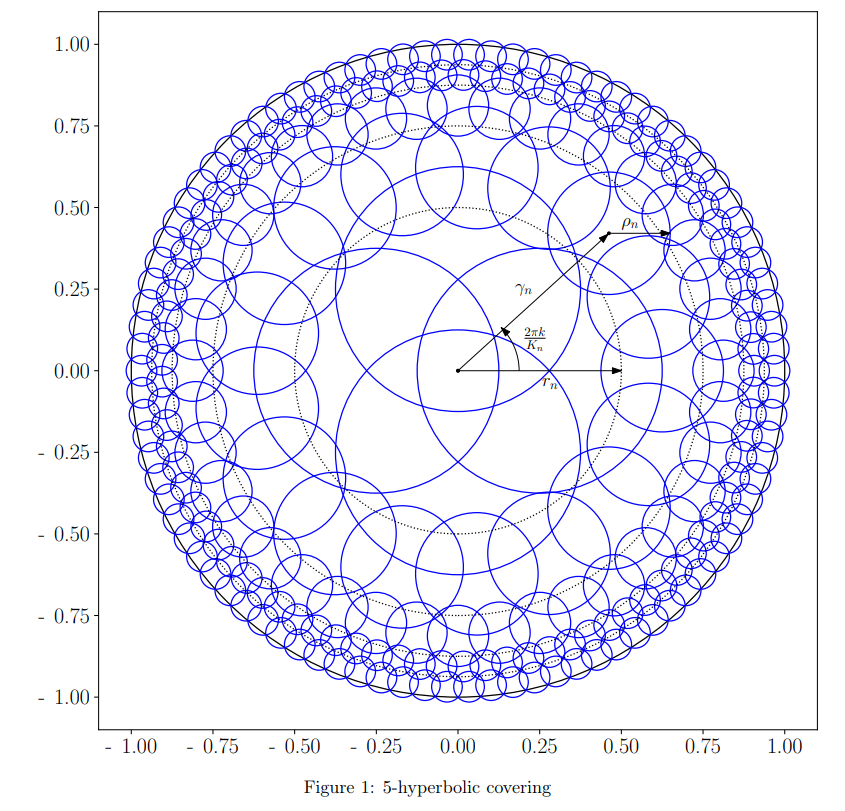
\includegraphics[scale=0.25]{Project Files/hyperbolic-cover.png}
        \label{fig:enter-label}
    \end{figure}
    % 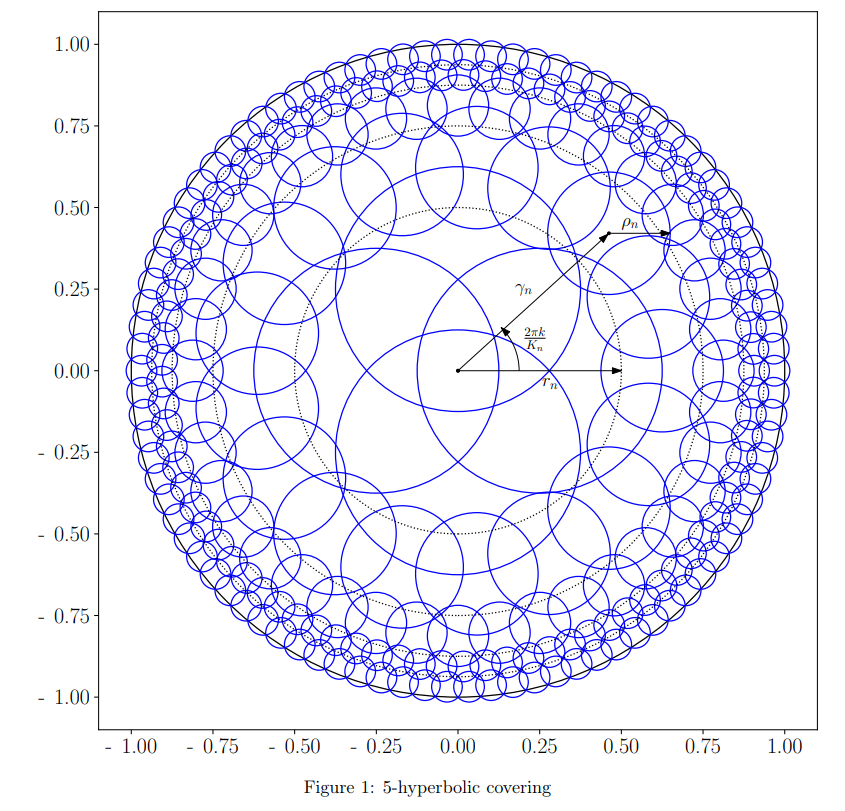
\includegraphics[scale=0.25]{Project Files/hyperbolic-cover.png}

    \blfootnote{[Mor21]}
\end{frame}

\begin{frame}{m-hyperbolic Approximation}
    Given a polynomial of degree d with $\lVert f \rVert \le 2^\tau$, and an integer $m > 1$, an m-hyperbolic approximation $H_{d, m}$ of f is a finite set of pairs $(g, a)$ where g is an m degree polynomial, and a is an affine transformation such that:
    \begin{itemize}
        \item The set of disks $a \left(D(0, 1)\right)$ is the N-hyperbolic covering, with $N = \lceil \log_2 \left(\frac{3ed}{m} \rceil \right)$, i.e., $a(X) = \left(\gamma_n + \rho_n X\right) e^{2 \pi i \frac{k}{K_n}}$
        \item $\lVert f \circ a - g \rVert \le 3 \lVert f \rVert 2^{-m}$
    \end{itemize}

    \blfootnote{[Mor21]}
\end{frame}

\begin{frame}{Number of disks}
    \begin{block}
        {Lemma} Given two integers d and $m > 1$, let $N = \lceil \log_2 \left(\frac{3ed}{m} \rceil \right)$. Then, the number of disks in the N-hyperbolic covering is in $O(d/m)$ and the union of the disks contains the unit disk.
    \end{block}

    \begin{block}
        {Proof}
        Total number of disks $t = \sum_0^{N-1}K_n$ \\
        We have $K_n \le 2^{n+4}$, $\Rightarrow t \le 2^{N=4} \le 16 \cdot 3e \frac{d}{m}$ \\
        Therefore, $t = O(d/m)$

        CLAIM: For any ring $R_n = D(0, r_{n+1}) \setminus D(0, r_n)$, the union of disks centered at $\gamma e^{2 \pi i \frac{k}{K_n}}$ with radius $\rho_n$ contains $R_n$.
    \end{block}

    \blfootnote{[Mor21]}
\end{frame}

\begin{frame}{Approximation Algorithm}
    \begin{block}
    {Theorem}
        Given a polynomial f of degree d, and an integer $ m > 1$, the m-hyperbolic approximation of f can be computed in $\Tilde{O}\left(d(m+\tau)\right)$
    \end{block}
\end{frame}

\begin{frame}{Approximation Algorithm}
    \begin{figure}
        \centering
        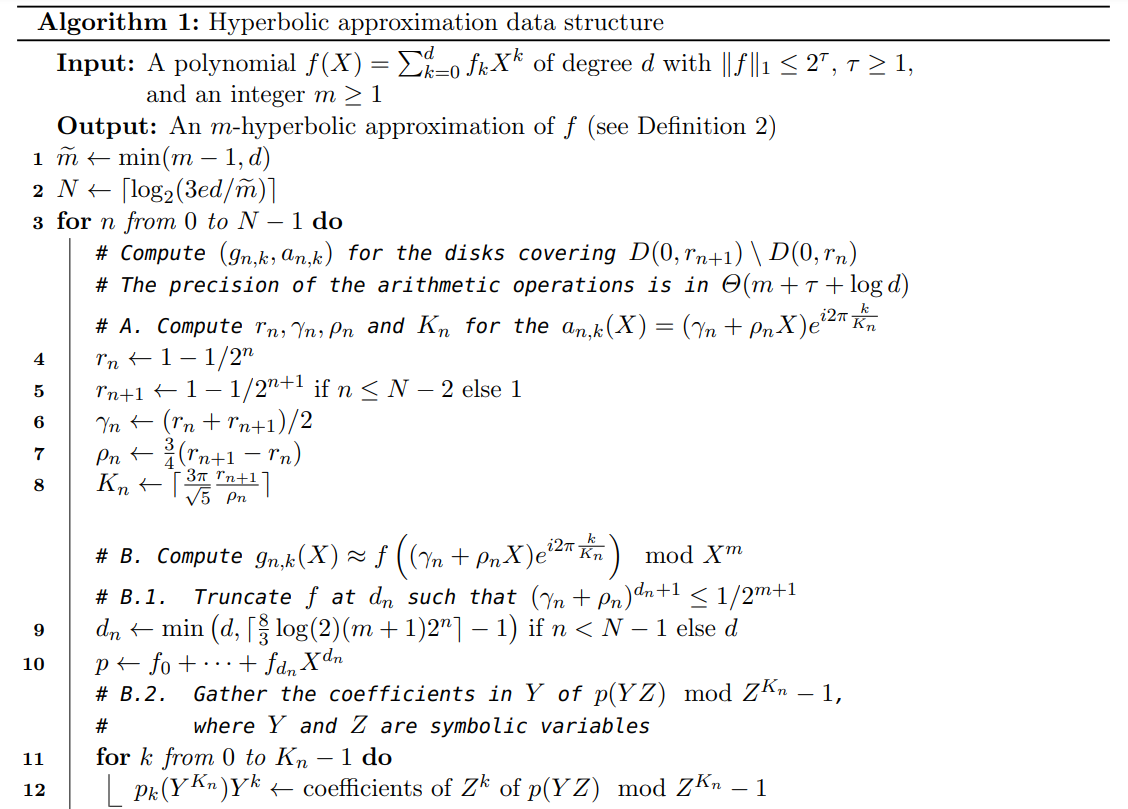
\includegraphics[scale=0.25]{Project Files/algo-1.png}
        \label{fig:enter-label}
    \end{figure}

    \blfootnote{[Mor21]}
\end{frame}

\begin{frame}{Approximation Algorithm}
    \begin{figure}
        \centering
        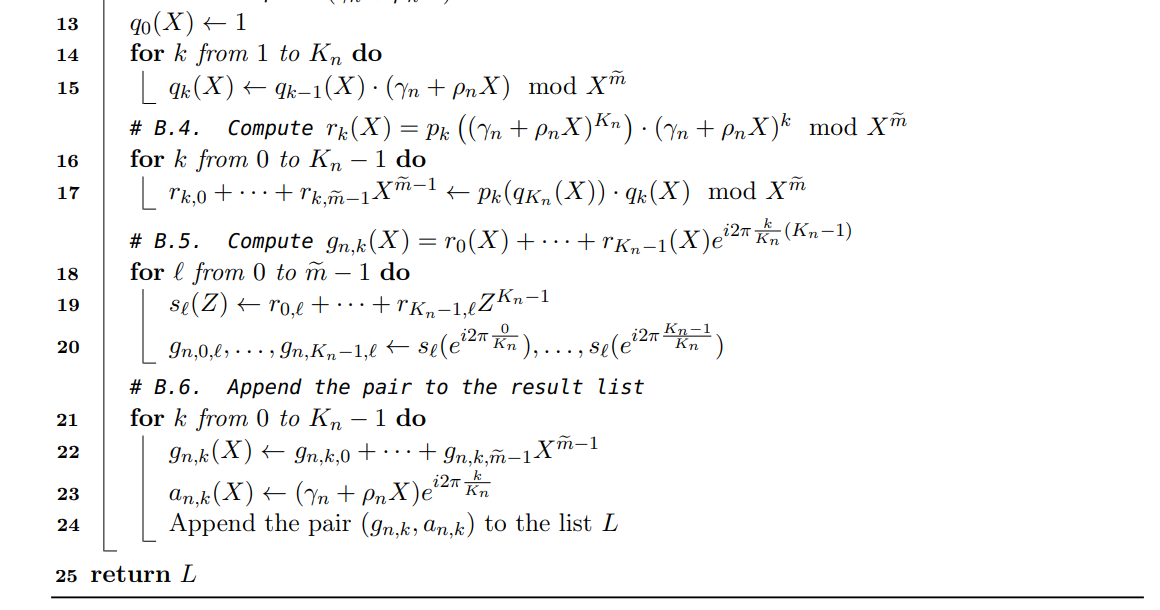
\includegraphics[scale=0.25]{Project Files/algo-2.png}
        \label{fig:enter-label}
    \end{figure}

    \blfootnote{[Mor21]}
\end{frame}

\begin{frame}{Overall Algorithm}
    \begin{algorithm}[H]
    \SetAlgoLined
    \KwData{polynomial f of degree d, d numbers $x_i \in D(0,1)$, precision m}
    \KwResult{List of evaluations $y_i$ such that $\lvert y_i - f(x_i) \rvert \le \lVert f \rVert 2^{-m}$}
        $L \leftarrow \{\}$ \\
        $Q \leftarrow$ data structure constructed from $x_i$, for fast disk range search \\
        $G \leftarrow H_{d, m+2}(f)$ \\

        \For{$(g_k, a_k)$ in G}{
        $v_1, \cdots v_{n_k} \leftarrow$ query Q for range $a_k$ \\
        $y_1, \cdots y_{n_k} \leftarrow g_k\left(a_k^{-1}(v_1)\right) \cdots g_k\left(a_k^{-1}(v_{n_k})\right)$ \\
        Append $y_1, \cdots y_k$ to L
        }
        \KwRet{$L$}\;
    \caption{\textsc{Approx-Multipoint-Eval} Algorithm}
\end{algorithm}
\end{frame}